Parallel to section \ref{sec:metsTorque}, we split this section into three pieces, first the results yielded by our sensor-circuit system calibration, then the in-lab work and at last the clinical findings.

\subsection{Sensor Calibration}
\label{sec:calResult}

% ============================================================
% APPENDIX E -- Torque Sensor Calibration Additional Results
% ============================================================

This appendix presents supplementary results from the torque sensor calibration process described in Section~\ref{sec:sensorCal}. The aluminum-based sensor was selected for all reported measurements based on its consistency and sensitivity relative to the other candidate materials. The figures here document the calibration trials for the glass and clear plastic sensors, which showed insufficient linearity and voltage range for reliable use. Together these results justify the sensor selection and positioning choices reported in Chapter~\ref{ch:matsNmets} and use for results presented in Chapter \ref{ch:results}.

The sensor calibration consisted in incrementally adding weight to our sensor as described in section \ref{sec:sensorCal}. The strain sensors studied included clear plastic, aluminum, and glass. Each sensor was tested for linearity voltage vs. weight up to 800 mg. Figure \ref{fig:rods5n7} shows calibration plots for two of the trials done. (a) The glass sensor showed some linearity, but small mean voltage range of operation even at max weight. The slope found for each fit is too different and non reproducible. (b) The clear plastic sensor showed stiffer,  showing better slope trend consistency but still being too uncertain.

These results demonstrated that these sensors were unreliable, and characterized by unpredictable changes in voltage when weight was applied. Additionally, both sensor had a sub-millivolt range, ineffective for measurements. These two rods were the thickest of all available rods in Table \ref{tab:rods}. The observed behavior is expected as explained by Equation \ref{eq:force_to_voltage}.


\begin{figure}[htb!]
	\centering
	
	\subfloat[\label{fig:glassRod5}]{
		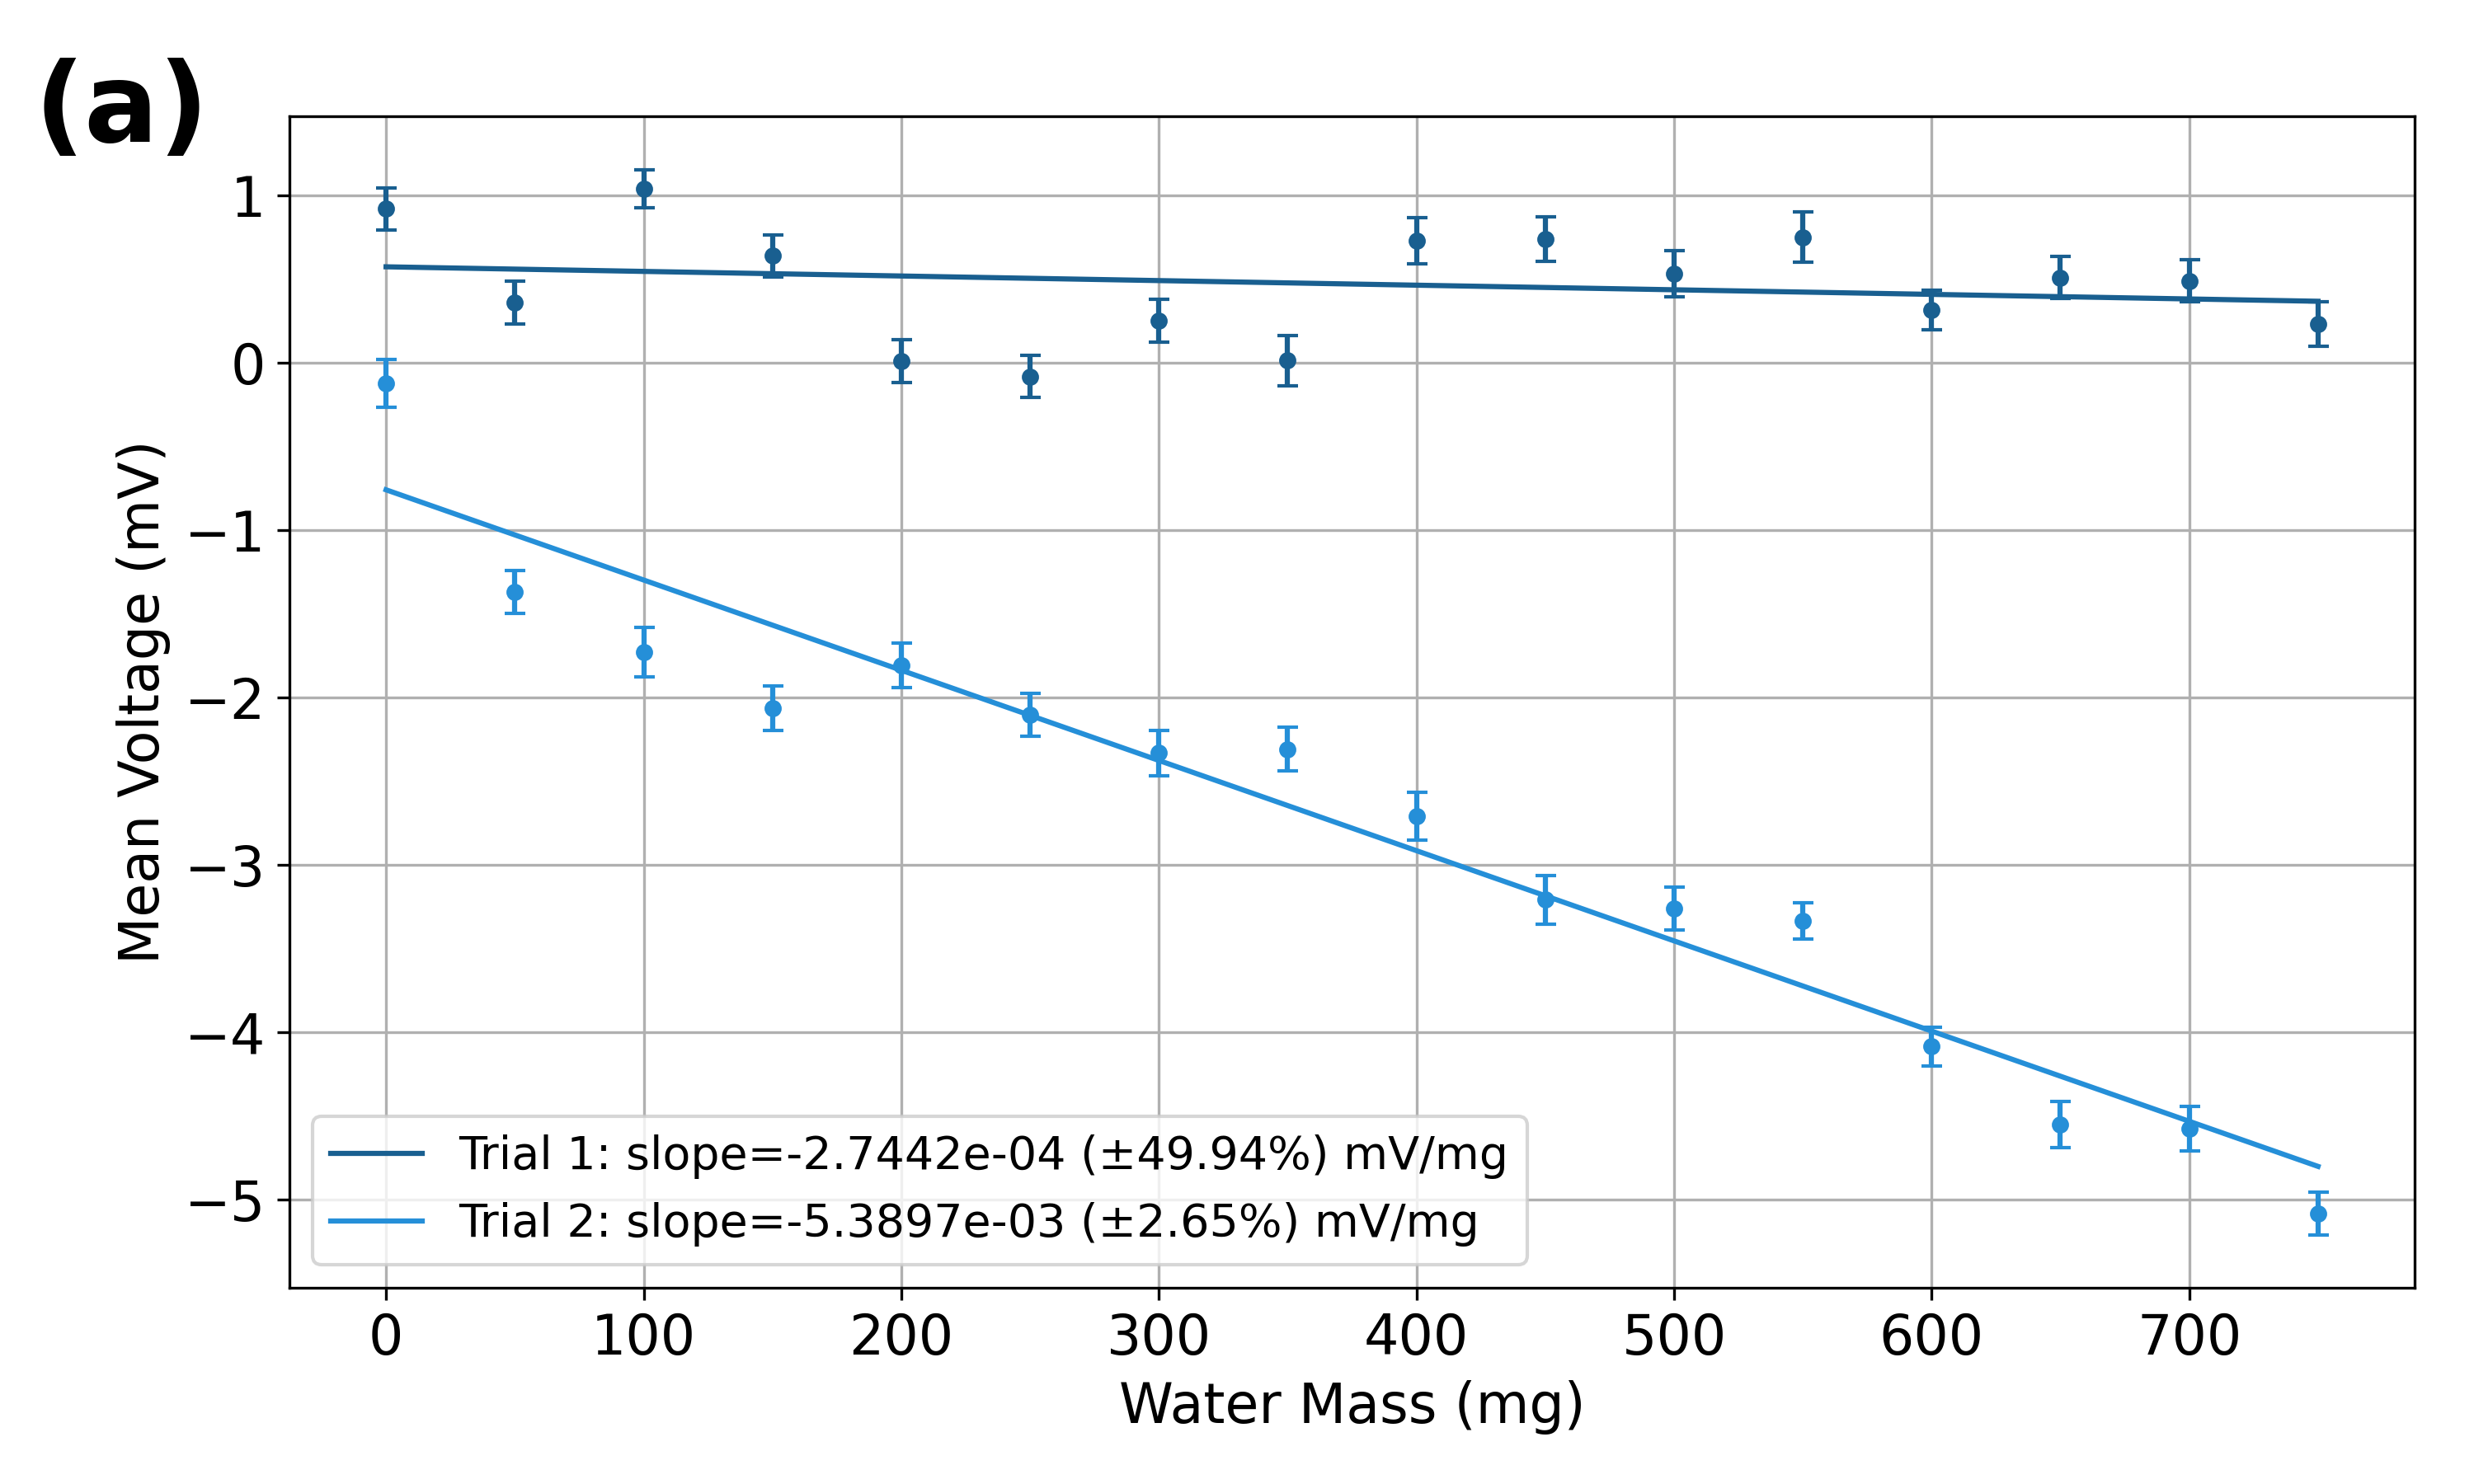
\includegraphics[width=\textwidth]{Assets/glass_fit.png}
	}
	\hfill
	\subfloat[\label{fig:clearRod7}]{
		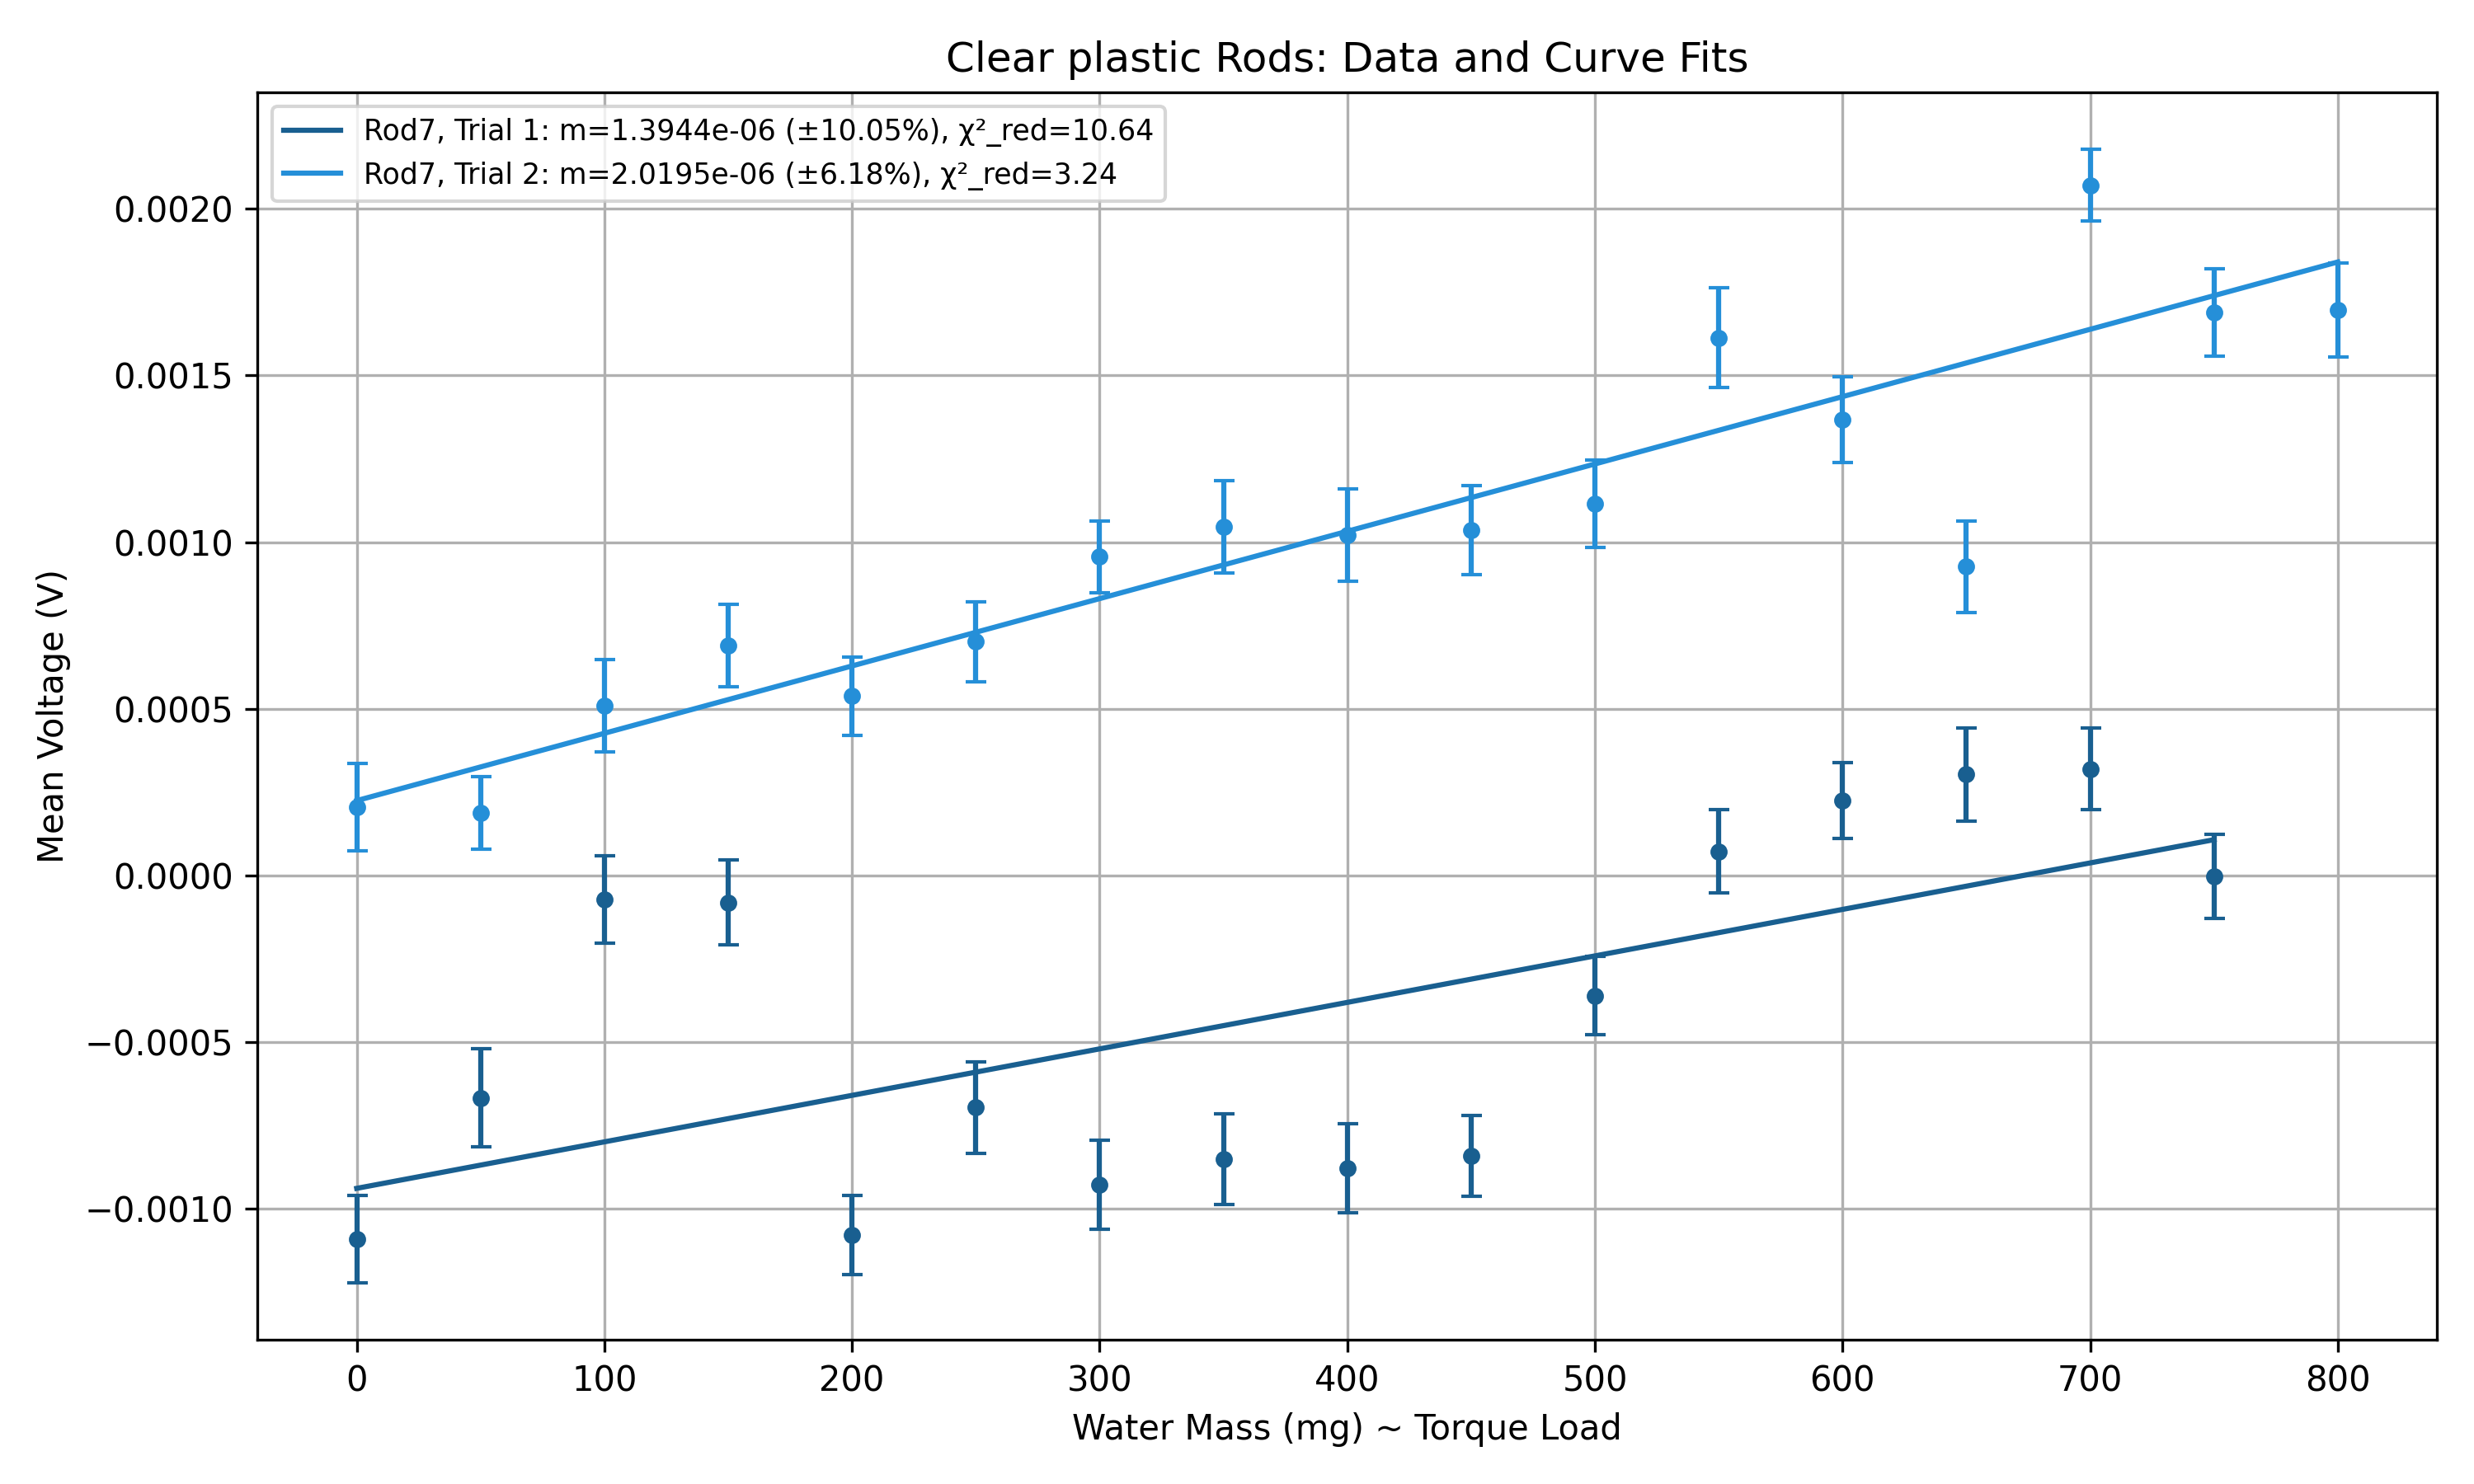
\includegraphics[width=\textwidth]{Assets/clear_plastic_fit.png}
	}
	\caption[Calibration trial results for low-torque rods showing poor sensor response]{Trial examples for Rods 5 and 7. Both of them showed inconsistency across trials showing minimal to no change in voltage with weight added. (a) Voltage readings for Rod5 (Glass) with up to 750 mg of water in increments. (b) Voltage readings for Rod7 (Clear Plastic) with up to 800 mg of water in increments.}
	\label{fig:rods5n7}
\end{figure}

In contrast the aluminum rods, 2 and 3, showed a clear linear trend along all trials and measurements (Figure \ref{fig:scaleCalb} ). This plot features three different sensor rotation configurations (Fig \ref{fig:cantileverConfigs}). Either 0$^\circ$ or 180$^\circ$ gave maximum deformation of the strain gauges, while 90$^\circ$ was ineffective.

\begin{figure}[htb!]
	\centering
		\subfloat[\label{fig:linearfitAlrods}]{
		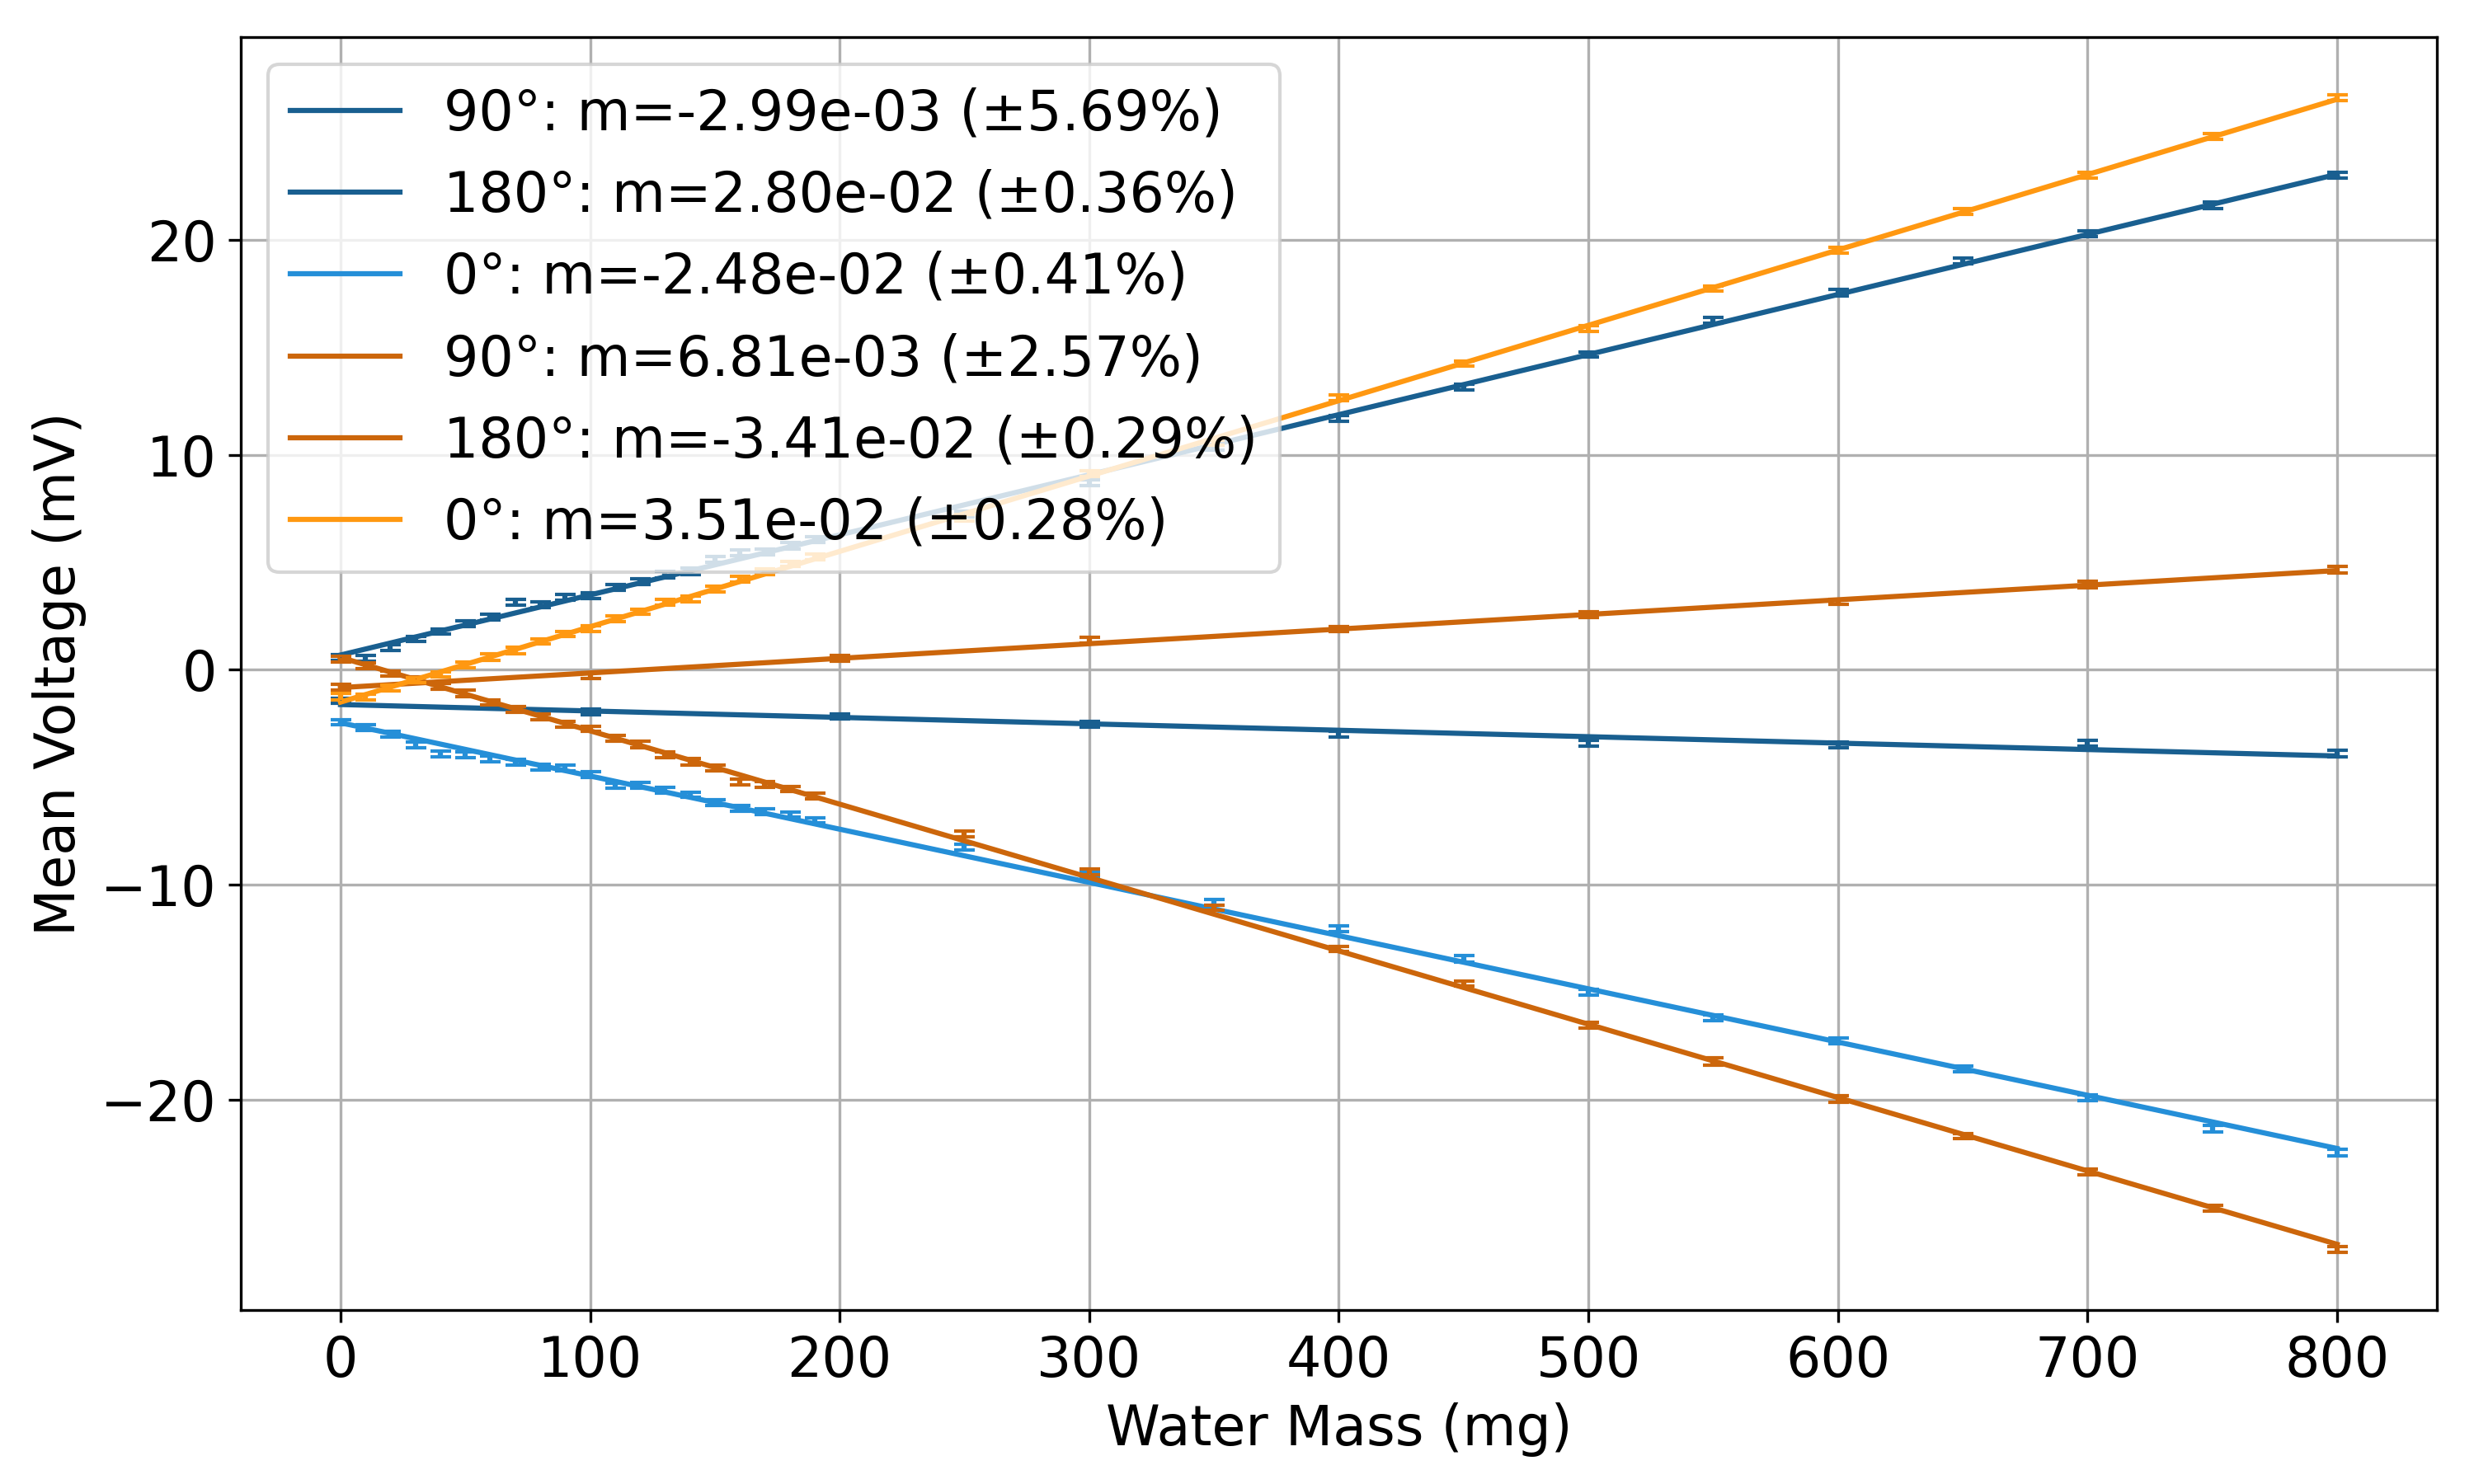
\includegraphics[width=0.95\textwidth]{Assets/al_fit.png}
	}
	\hfill
		\subfloat[\label{fig:cantileverConfigs}]{
		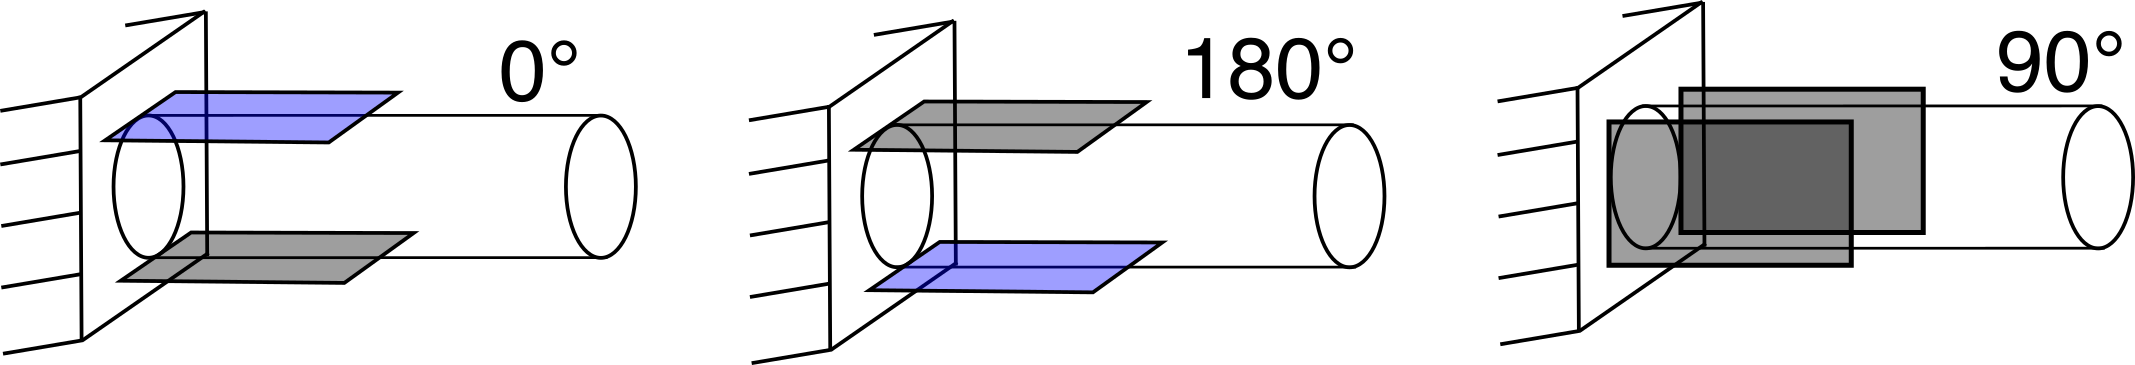
\includegraphics[width=0.85\textwidth]{Assets/calConfigs.png}
	}
	\caption[Orientation Response of cantilever sensor during calibration.]{Linear fits show consistent response across orientations, confirming the reliability of the lab-built sensor. (a)Calibration curves for two aluminum (AL) rods in three different orientations. (b)Three configurations tested, 0$^\circ$ and 180$^\circ$ are equivalent but flip voltage sign with respect of each other. 90$^\circ$ gives less sensibility as strain gauges does not bend in the proper axis.}
	\label{fig:scaleCalb}
\end{figure}

From these results, we used rod 3 oriented in either 0 or 180 degrees, since it showed remarkable consistency across calibration trials. Focusing on the weight range(0 to 200 mg), we found similar slopes in repeated calibrations over a period of one week.

Figure \ref{fig:posAndHeight} shows two lines, along the lever arm 90 and 50 mm ($r$) away from the rotation axis position. On the x-axis position along the sensor length measurements demonstrated greater sensitivity for greater distances from the strain gauges. And we can see that the 50 mm line deviates from the 90 mm line showing that the closest to the rotation axis, the higher the signal reading for the same force.

\begin{figure}[htb!]
	\centering
	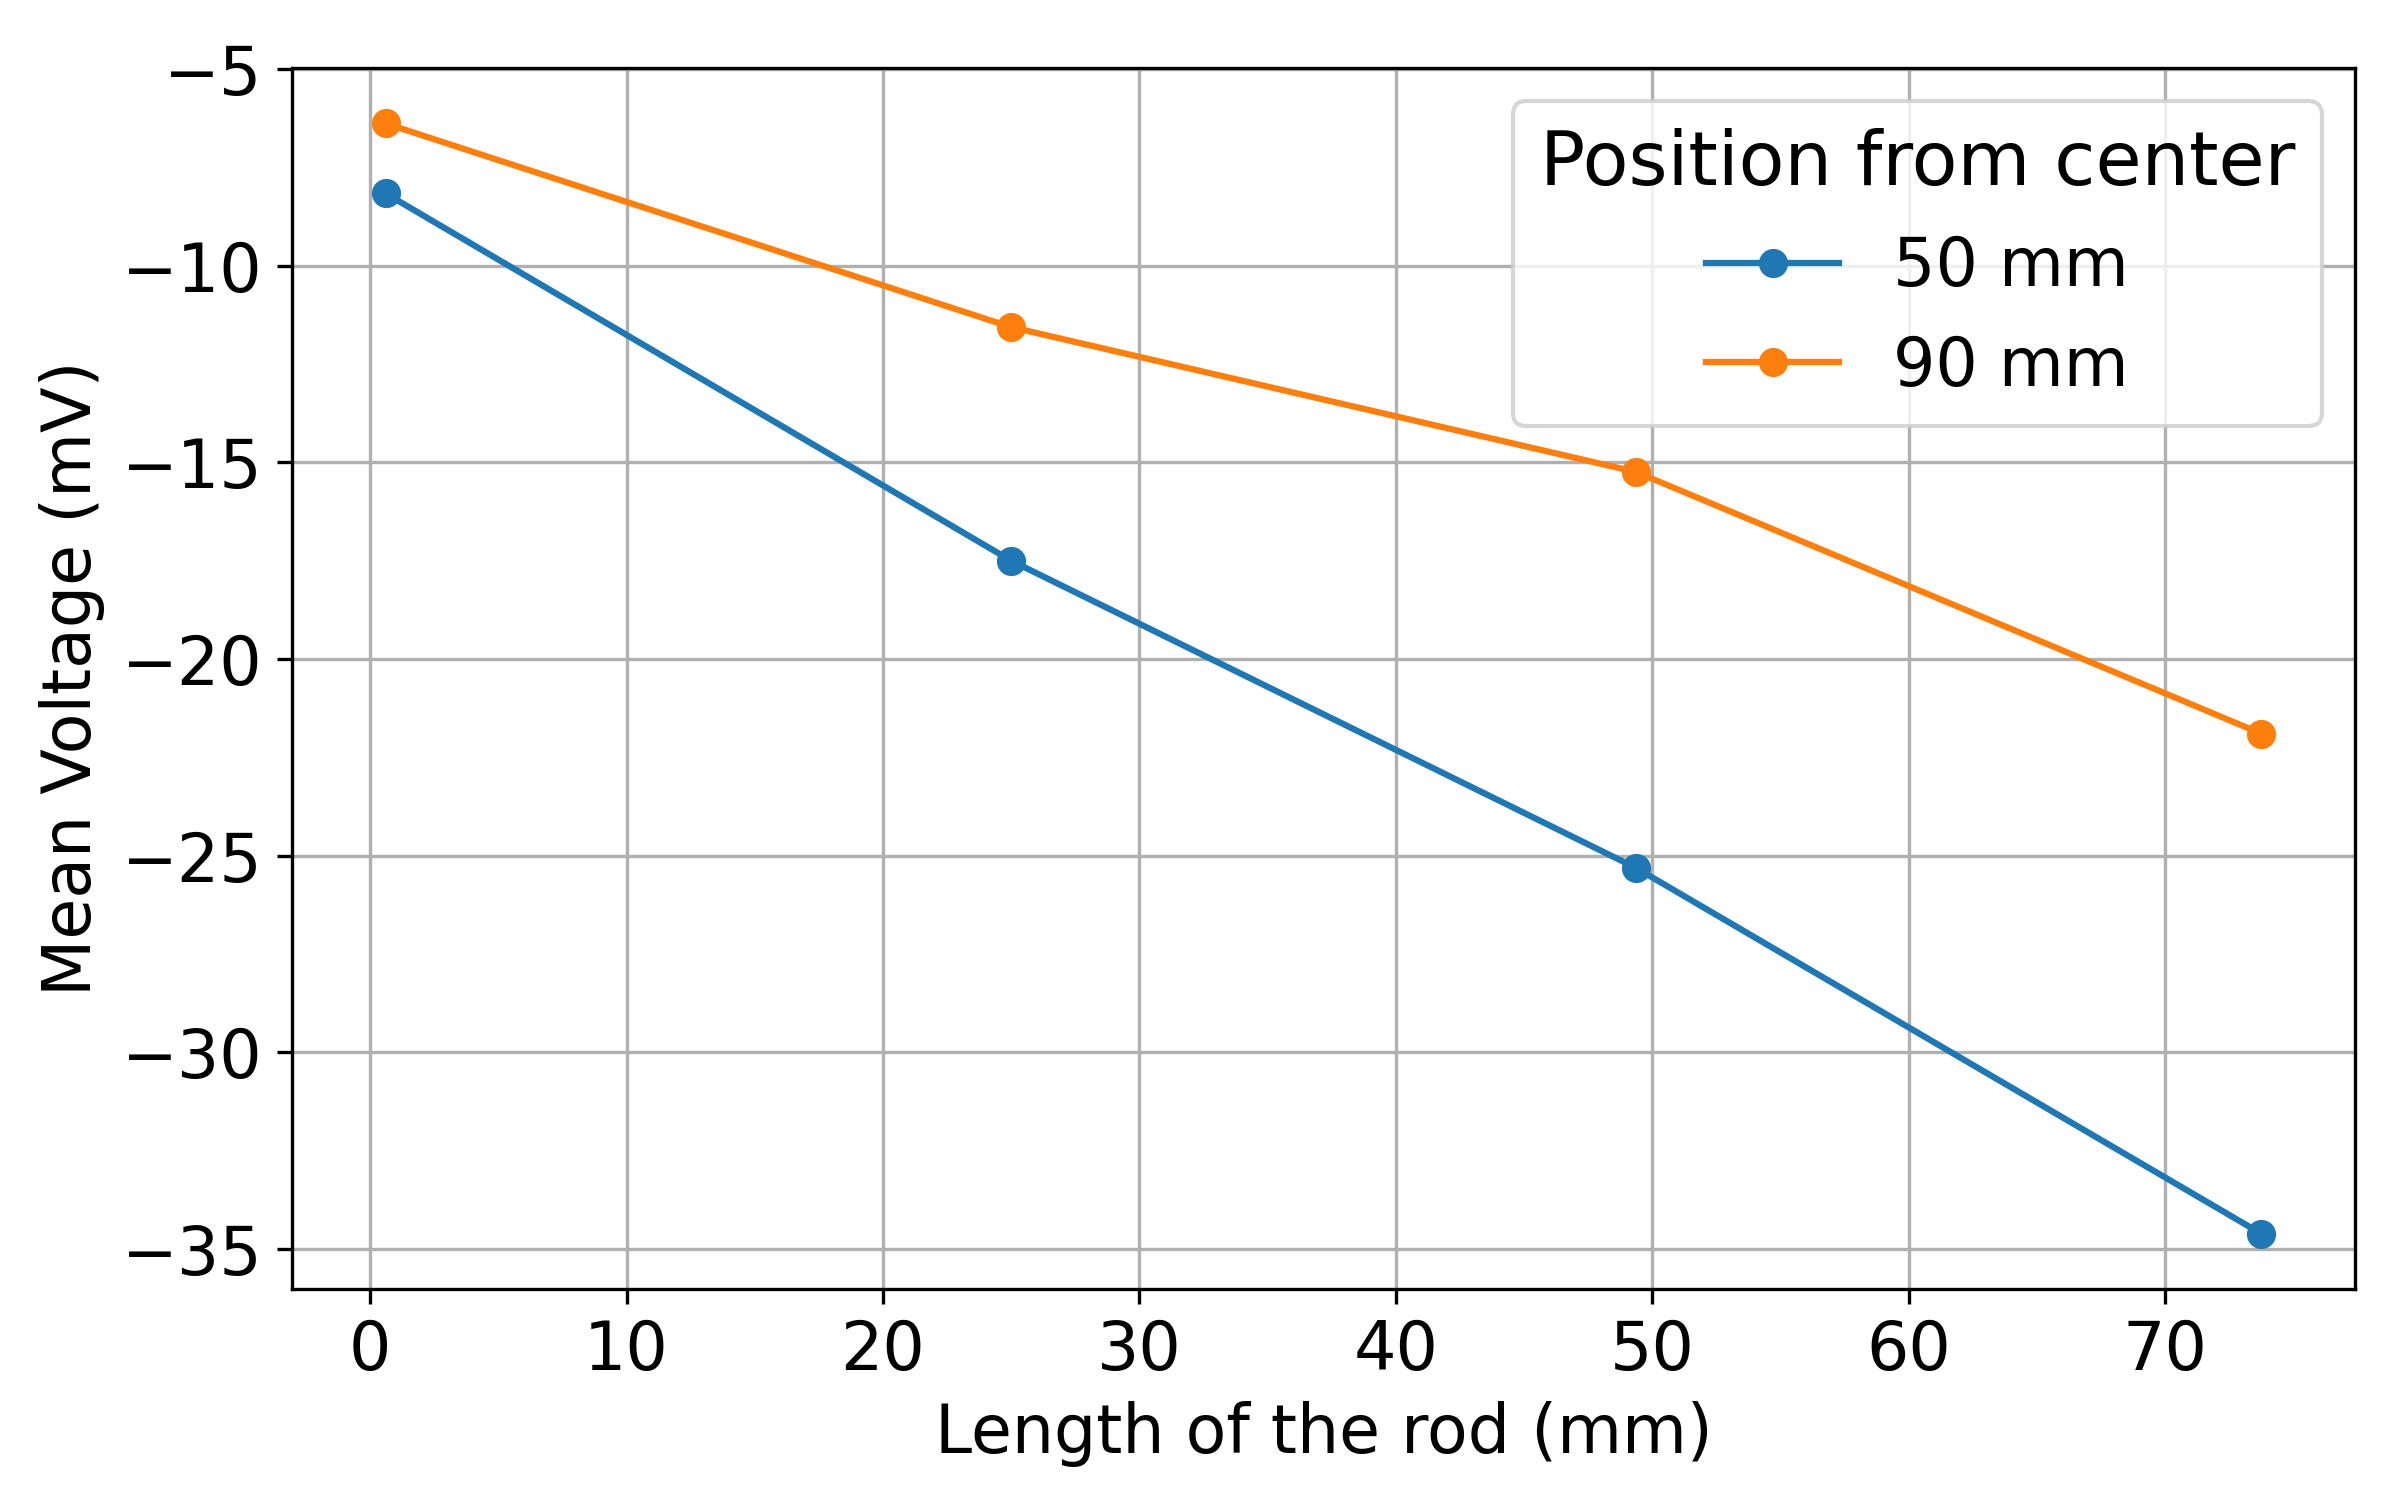
\includegraphics[width=0.85\textwidth]{Assets/1stTrials_50_90.png}
	\caption[Effect of sensor position on mean sensor voltage response]{Mean voltage response of the sensor as a function of length ($L$) for different distances  ($r$) from the center (50--90 mm). 
		At larger lengths (farther from the strain gauges) an increase in signal reading.
		Further from the rotation axis the measurements diverge, showing higher sensitivity near the center (50 mm). }
	\label{fig:posAndHeight}
\end{figure}

Figure \ref{fig:torque_fit} demonstrates the expected inverse relation of force and position along the transfer arm from the rotation axis ($1/r$) in two ways. First Figure \ref{fig:loglogtorque} shows a log-log plot voltage vs position with a fit n value very close to -1. Additionally, a $A/r$ fit (Figure \ref{fig:ABfittorque}) provides the constant $A$, also very close to -1. This signifies, it is a good method to measure torque via the counter force. 

\begin{figure}[hbt!]
	\centering
	
	\subfloat[\label{fig:loglogtorque}]{
		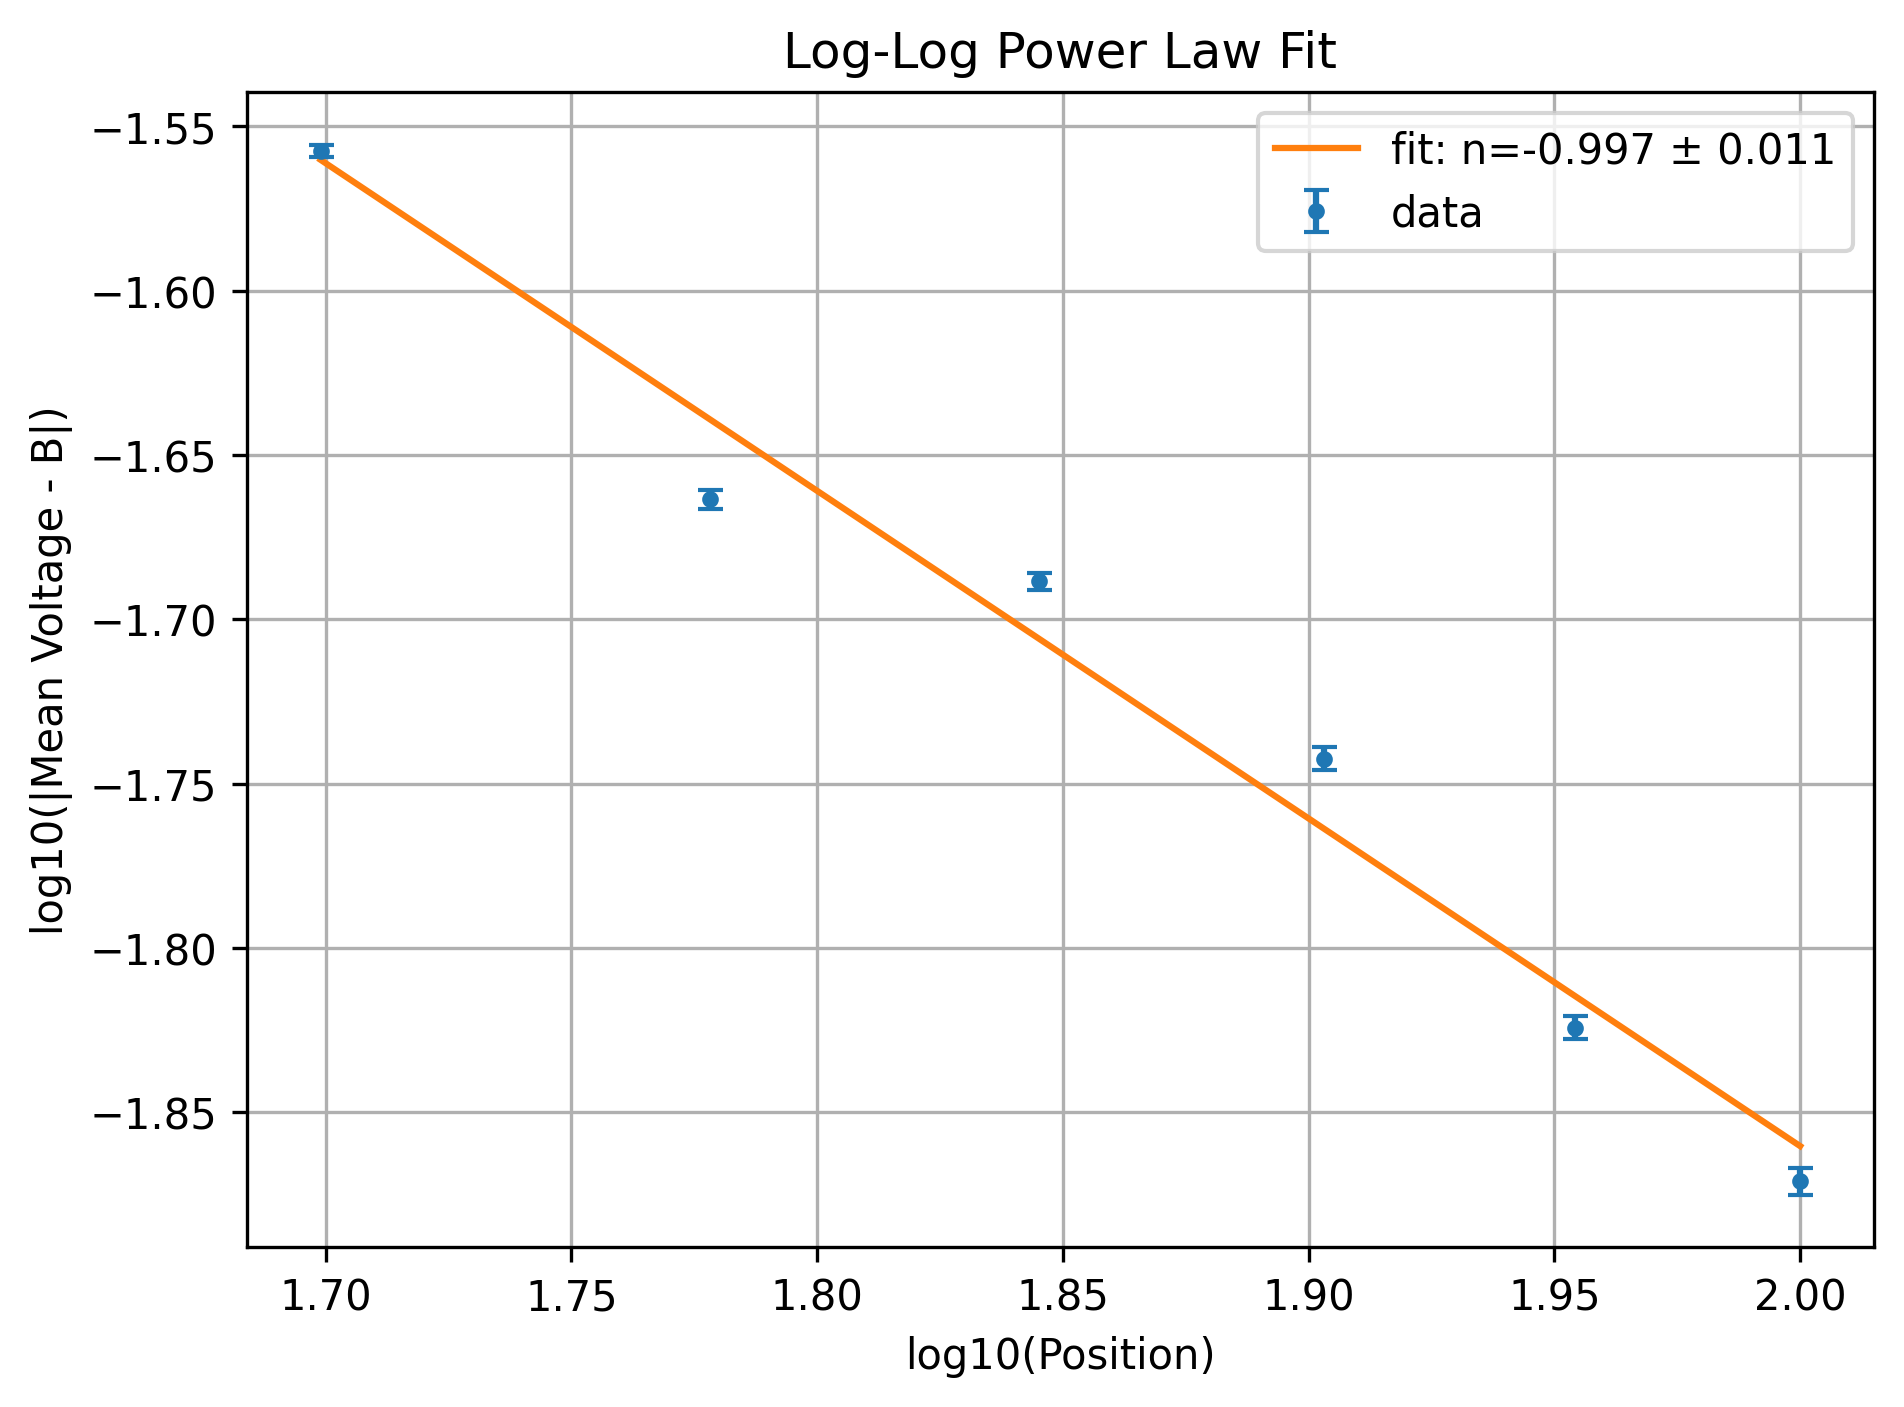
\includegraphics[width=0.85\textwidth]{Assets/powerFitFr.png}
	}
	\hfill
	\subfloat[\label{fig:ABfittorque}]{
		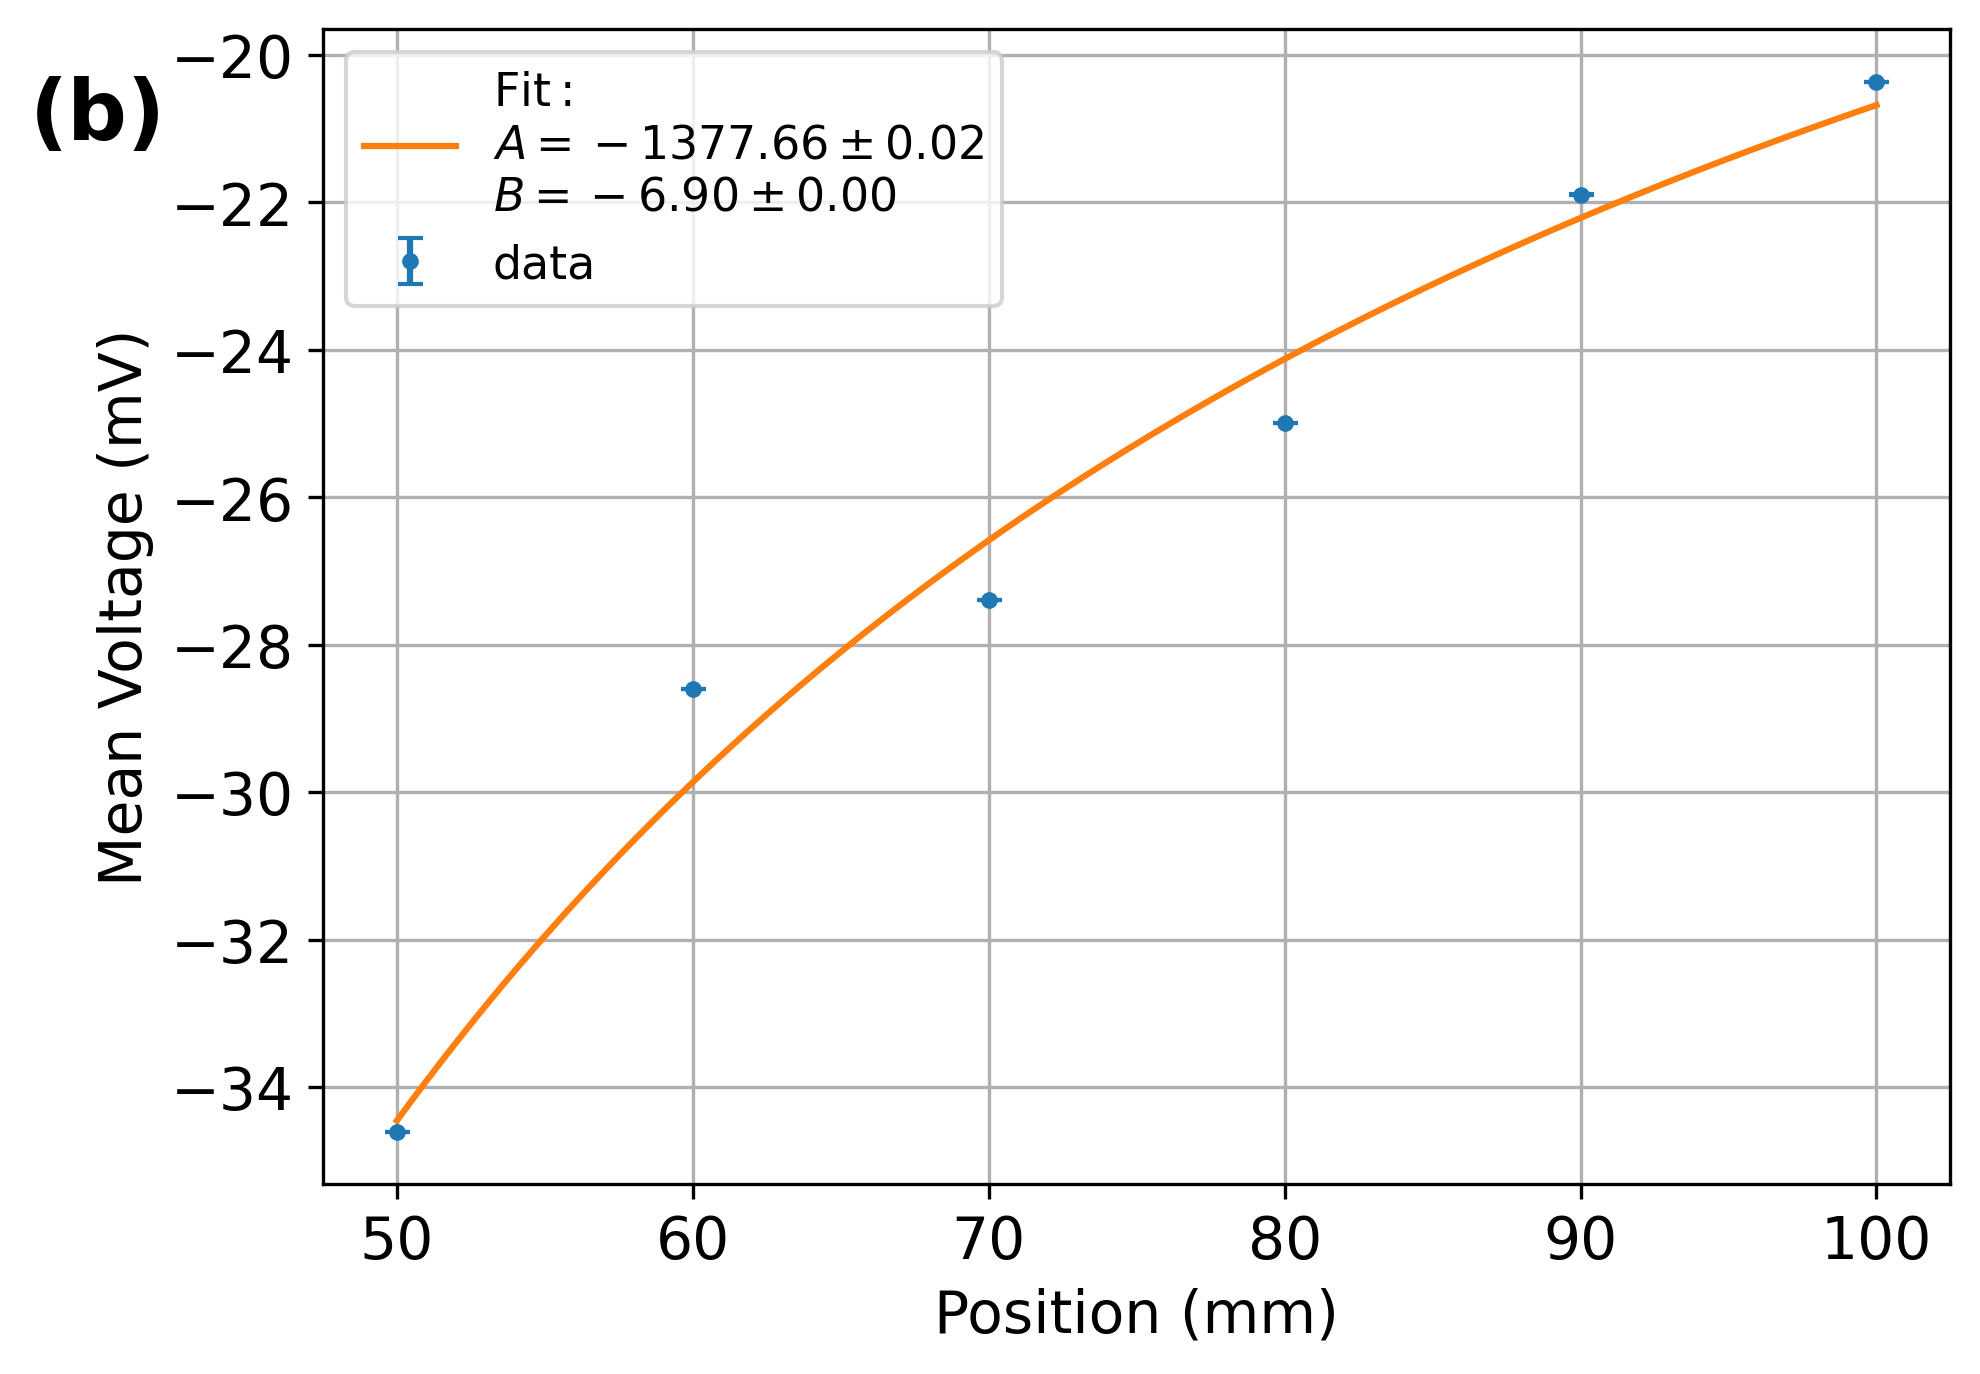
\includegraphics[width=0.85\textwidth]{Assets/inverseRfitFr.png}
	}
	\caption[Expected $1/r$ dependence of torque]{Demonstration of the expected inverse-distance dependence of the force (and thus torque) with respect to the distance $r$ from the rotation axis. Both analyses confirm the $1/r$ dependence characteristic of the torque measurement via counter-force method. (a) Log-log plot of effective measured voltage (proportional to force) versus position $r$, showing a power-law fit with exponent $n = -0.997 \pm 0.011$, very close to the theoretically expected value of $-1$. (b) Direct fit of the form $F(r) = A/r + B$, yielding $A = -1.378 \pm 0.015$ (very close to $-1$ in normalized units) and a negligible offset $B = -0.0069 \pm 0.0002$.}
	\label{fig:torque_fit}
\end{figure}

Once the sensor and circuit were calibrated and the best position for measurement in the torque fixture are affixed, we moved on to the in laboratory measurements of torque in Section \ref{sec:sensorCal}. 

\FloatBarrier

\subsection{Torque from Lab scale magnet}

As described in section \ref{sec:InLab_Torque}, torque measurements were performed under three different experimental configurations. When a small uniform magnetic field was applied using Helmholtz coils, the torque produced by the short (2 cm) magnetic dowel remained at or below the detection limit of the measurement system. For that reason, only the longer rod yielded reliable results. Figure \ref{fig:torque_longerRod} shows the maximum torque (N m) against the magnetic flux experimental data (in blue) exhibiting a clear parabolic dependence on $  B  $.

\begin{figure}[htb!]
	\label{fig:torque_longerRod}
	\centering
	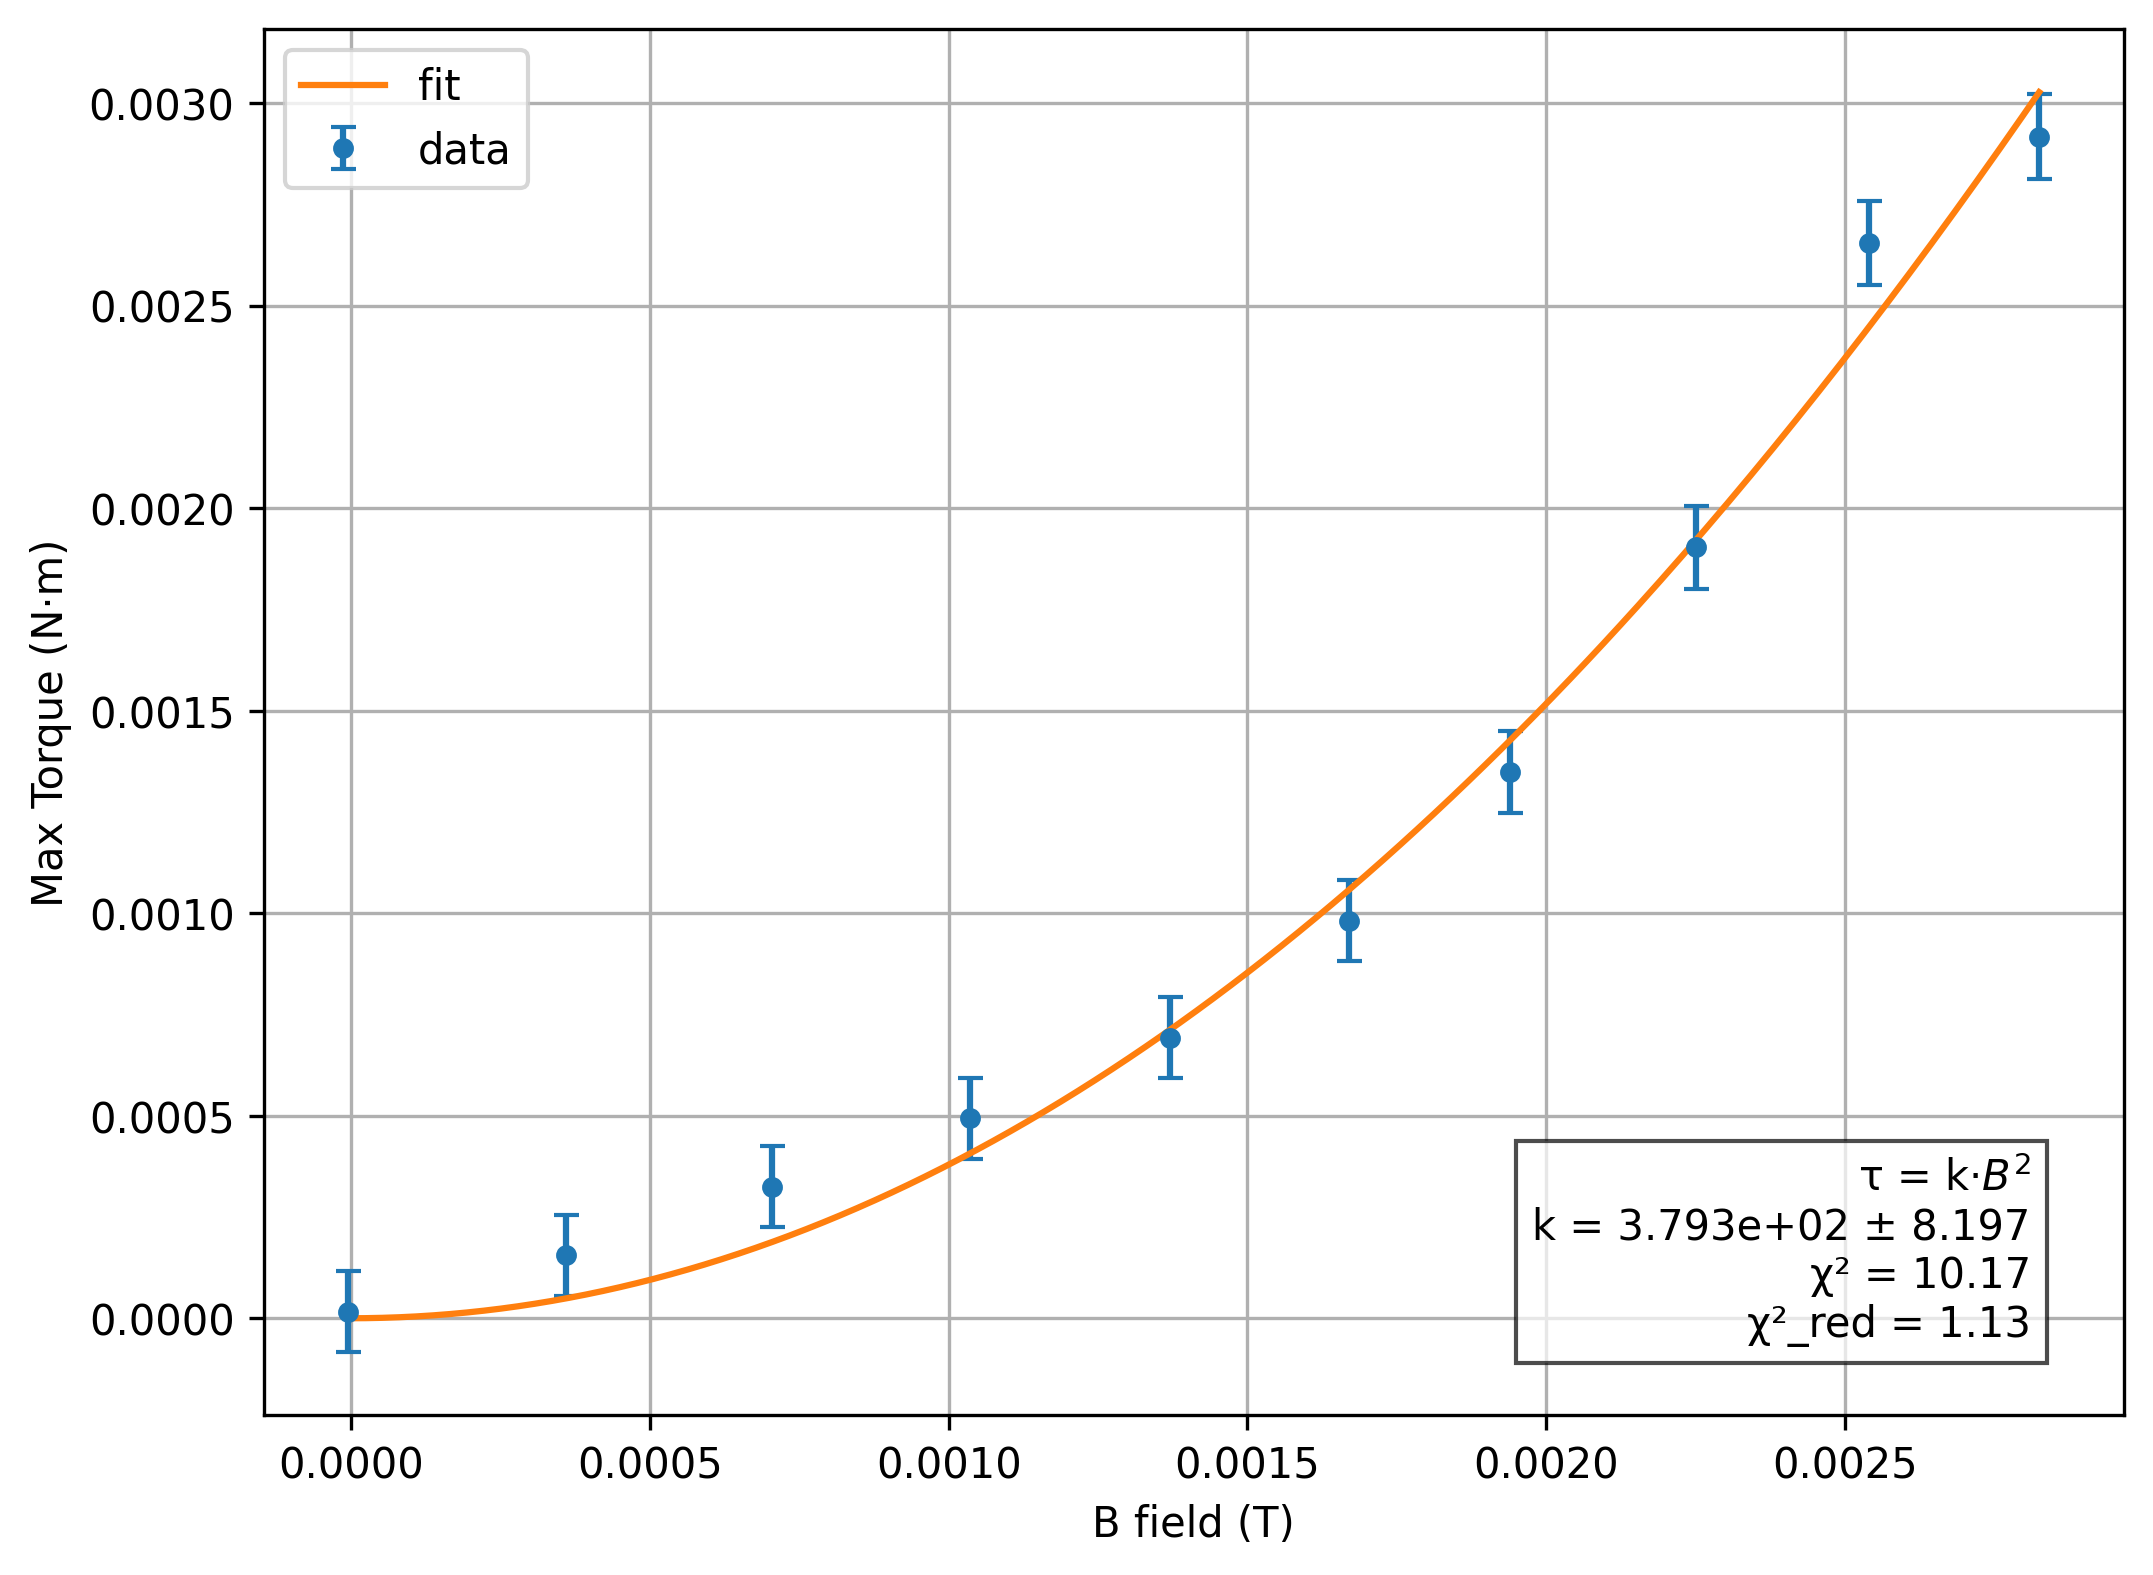
\includegraphics[width=0.85\textwidth]{Assets/example_plot.png}
	\caption[Torque vs. magnetic field strength for the longer rod under Helmholtz coils]{Maximum measured torque in Nm as a function of applied magnetic flux density in B for the longer rod under a Helmholtz coil configuration.}
\end{figure}

From the fit parameters, $k = 3.87 \pm 44.5$, $b = -5.56\times10^{-2}$ and $V_0 = 8.45 \times 10 ^{-5}$. The dominant quadratic term ($  k B^2  $) is in excellent agreement with the theoretical expectation for the torque on a magnetic dipole in a uniform field, where $  \tau \propto B^2  $. The linear coefficient $  b  $ is very small and statistically consistent with zero within uncertainty, while the offset $  V_0  $ is negligible, confirming the absence of significant systematic bias in the measurement.


A second set of measurements was performed on the shorter (2,cm) magnetic dowel using significantly stronger magnetic fields generated by four neodymium magnets. Figure \ref{fig:torque_shorterRod} shows a parabolic relationship, however the values on torque are smaller for higher magnetic fields 

\begin{figure}[htb!]
	\label{fig:torque_shorterRod}
	\centering
	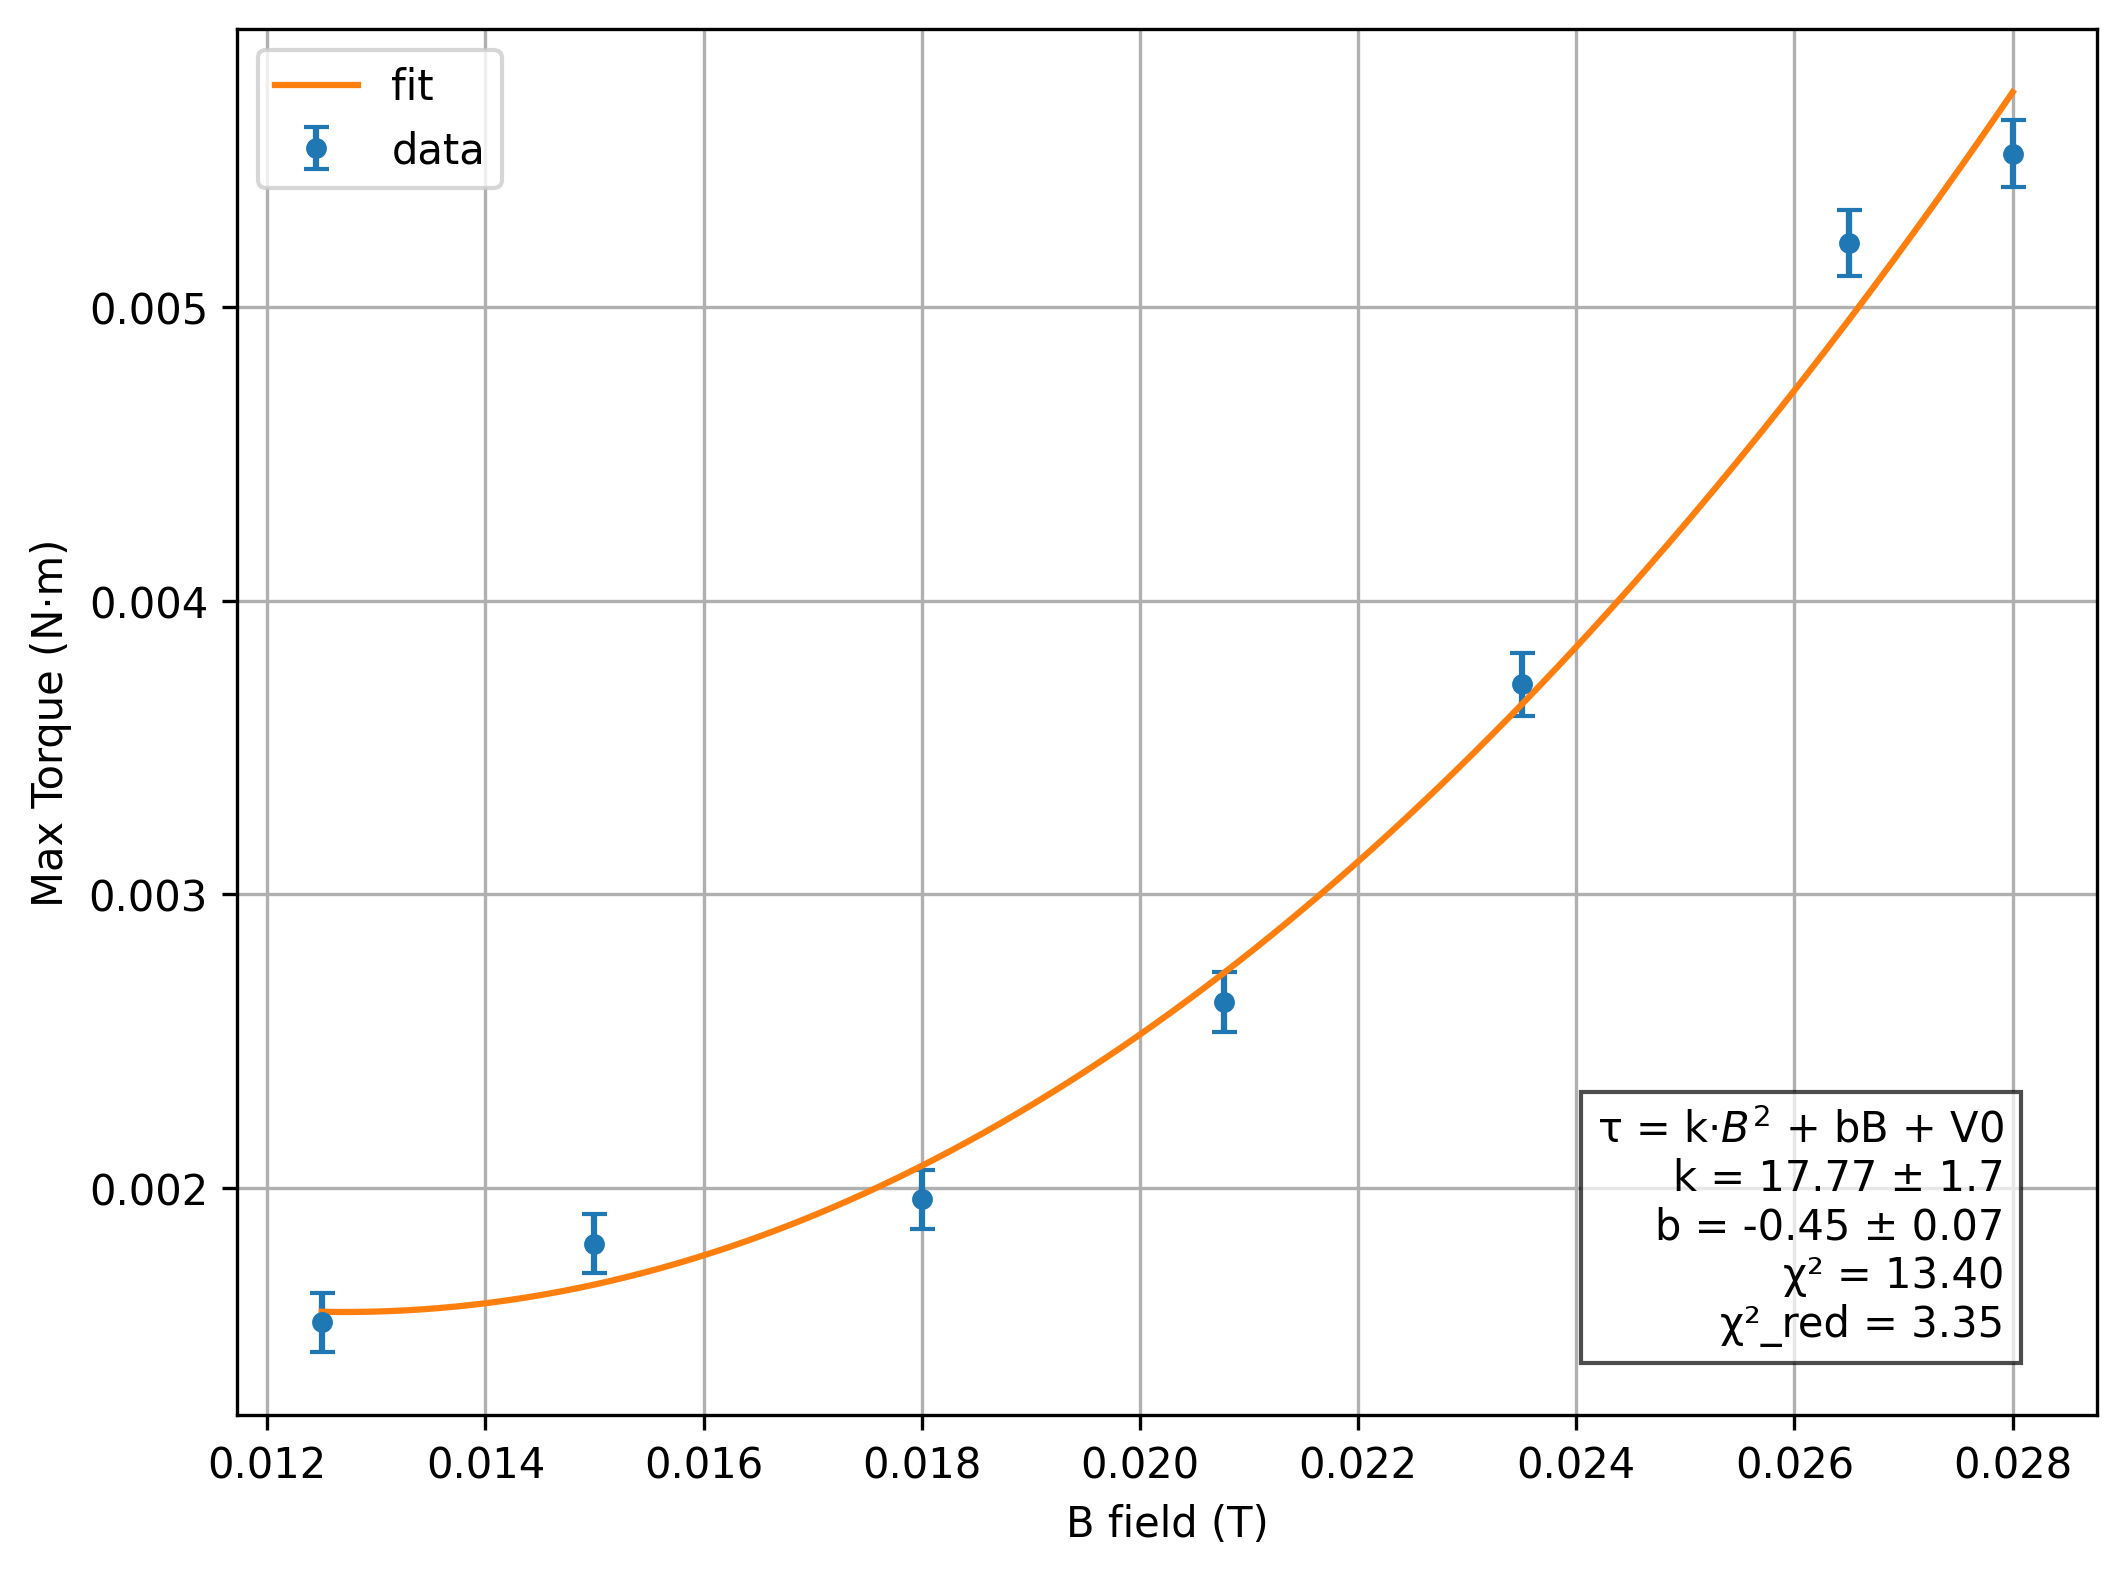
\includegraphics[width=0.85\textwidth]{Assets/example_plotS.png}
	\caption[Torque dependence on magnetic field strength for 2 cm rod under neodymium magnet fields]{Maximum torque in Nm as a function of applied magnetic flux density in T for the shorter (2cm) magnetic rod under stronger uniform fields (Neodymium magnets). Blue points is the experimental measurements while orange curve represents a quadratic fit}
\end{figure}

This time the fit yielded, 

\subsection{Torque from 3T Siemens Magnetom\textsuperscript{\texttrademark} \gls{mri} scanner}

Once in a clinical environment, both the circuit and the \gls{mri}-safe torque measuring fixture were functioning properly and circuit calibration was appropriate for clinical measurements. 

After a single session in the \gls{mri} room no torque was perceived. Neither test material shown any perceptible or measurable torque inside the scanner. 

Despite these efforts, no measurable torque-induced deflection or angular shift was detected on the sensor readout for either material.

The 316L stainless steel rods were found to be too short or too thin to generate detectable torque under the prevailing fringe-field conditions, indicating that longer segments, greater mass, or increased ferromagnetic contribution would be necessary to elicit observable effects in future iterations. Titanium rods likewise produced no response, aligning with expectations for its weakly paramagnetic properties in clinical \gls{mri} environments.

In total, several positioning attempts were made at central and progressively closer locations to the bore, but no quantifiable torque data could be obtained. The protocol ultimately failed to yield reliable torque measurements due to insufficient induced effect on the tested sample configurations. These observations highlight the need for more substantial material samples in subsequent testing to amplify any potential torque for characterization. 

\FloatBarrier